\important{Focus sur: le panneau solaire}

\begin{center}
    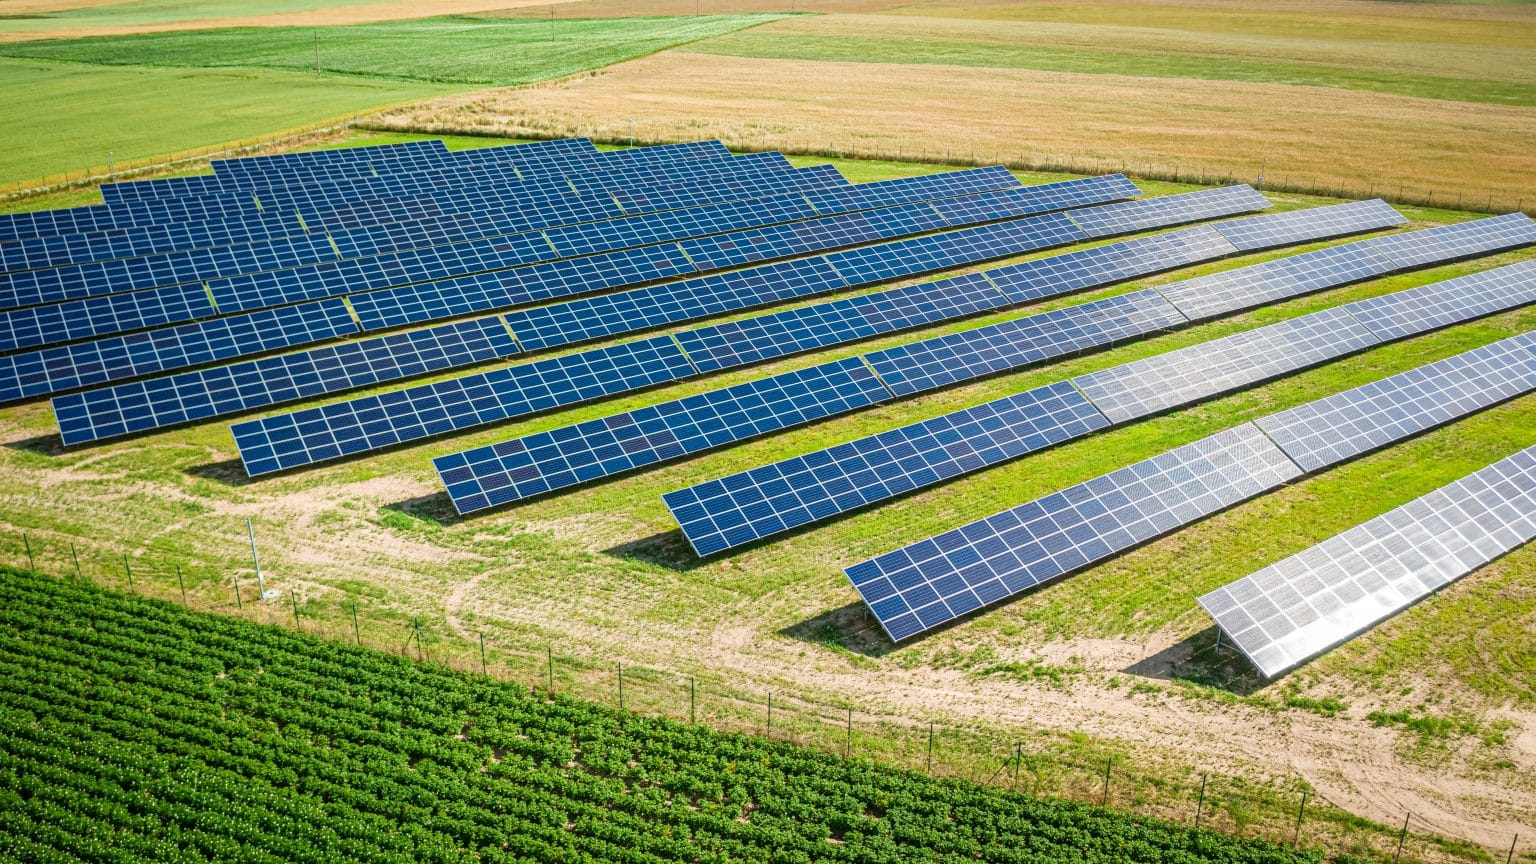
\includegraphics[width=8cm]{images/panneau solaire.jpg}

    \textit{Ferme solaire photovoltaïque}
\end{center}


Un panneau solaire est un dispositif qui permet de produire de l'électricité à partir de la lumière du Soleil. Il est composé de cellules photovoltaïques, le plus souvent de couleur bleu foncé, qui transforment directement la lumière en électricité.
Contrairement aux autres moyens de production, le panneau solaire ne possède pas d'alternateur : il n'y a aucune pièce en mouvement.
Pour produire beaucoup d'électricité, on installe souvent un grand nombre de panneaux sur un même terrain : c'est ce qu'on appelle une ferme solaire ou une centrale solaire.

Le panneau solaire utilise la lumière du Soleil, une source d'énergie renouvelable, et ne rejette pas de CO\textsubscript{2}. La production d'électricité dépend de la météo et du moment de la journée : elle est nulle la nuit et faible quand le ciel est couvert.
Une ferme solaire occupe une grande surface au sol, et la fabrication des panneaux nécessite des matériaux rares.